\section{Tests Environment and Results}

The previous section described how the system was implemented and how each
component interacts within the complete flow, from a user that uploads a file to
the leader performing the Corruption Check phase (showed in Section
\ref{sec:check-corruption}).

This section presents the testing environment, the scenarios used during evaluation, and the obtained results. The tests were executed on a cluster of nine machines running Ubuntu 24.04.1 LTS (GNU/Linux 6.8.0-51-generic x86\_64). The specifications of the virtual machines are summarised in Table \ref{tab:vms-specs}. The nodes were geographically distributed across the European continent.

\begin{table}[h!]
    \centering
    \begin{tabular}{|l|c|c|c|c|}
    \hline
       \textbf{Node ID} & \textbf{IPv4} & \textbf{CPU(s)} & \textbf{RAM} & \textbf{Disk} \\
       \hline
        GW & 51.15.221.121 & 8 & 32 GB & 45 GB \\
        agent 1 & 212.47.241.22 & 4 & 16 GB & 45 GB \\
        agent 2 & 51.15.138.169 & 4 & 16 GB & 45 GB \\
        agent 3 & 51.159.178.75 & 4 & 8 GB & 45 GB \\
        agent 4 & 51.158.75.32 & 4 & 8 GB & 45 GB \\
        agent 5 & 51.158.233.202 & 4 & 8 GB & 45 GB \\
        agent 6 & 51.15.108.2 & 4 & 8 GB & 45 GB \\
        agent 7 & 151.115.42.176 & 4 & 8 GB & 45 GB \\
        agent 8 & 151.115.104.48 & 4 & 8 GB & 45 GB \\
        \hline
    \end{tabular}
    \caption{Specifications of the machines used in the testing environment.}
    \label{tab:vms-specs}
\end{table}

Each test scenario considered four parameters:
\begin{itemize}
    \item \textbf{Number of agents}: total number of agents participating in the Reed-Solomon configuration of $n + k$ nodes.
    \item \textbf{Number of offline agents}: number of agents intentionally
        disconnected during the corruption check.
    \item \textbf{Number of files}: number of files included in the test.
    \item \textbf{File size}: size of each uploaded file. Since each file is divided into $n + k$ shards, the size of a single shard equals $\frac{\text{file size}}{\text{number of agents}}$ bytes.
\end{itemize}

All the scenarios consider that some agents, respecting the Reed-Solomon
requirement, could be offline during the uploads. In these scenarios, the time of shard recovery described in Section~\ref{sec:recovery-of-missing-shards} was included. Once all files had been uploaded, the system was evaluated through the corruption check procedure. The total elapsed time, measured in seconds, was recorded from the initiation of the check until its completion. A test was deemed valid only if the system successfully detected file corruption. Each plotted value represents the average total elapsed time over three independent runs.

\paragraph{Test 1: Large files, all agents online}

In the first scenario, 100 files of 100 MB each were uploaded, yielding a total
dataset of 10 GB. Each file was divided into $n+k$ shards and distributed across
the agents in the cluster. All agents remained online during the corruption
check. Figure \ref{fig:test-1} shows the elapsed time for the corruption check
as the number of agents increases from 3 to 8. As expected, elapsed time grows
with the number of agents due to network delays. The elapsed time ranges from 1.373 seconds with 3 agents to 23.892 seconds with 8 agents. These results establish a baseline for moderate-size files, indicating that the system efficiently handles shard verification with minimal computational overhead.

\begin{figure}[!ht]
\centering
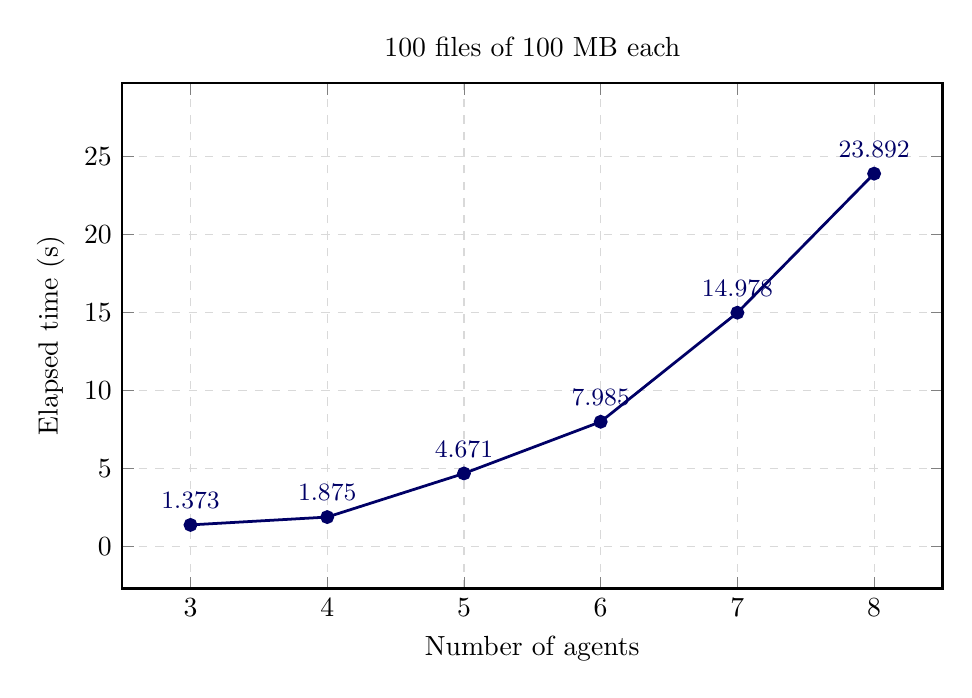
\begin{tikzpicture}
\begin{axis}[
    width=12cm, height=8cm,
    xlabel={Number of agents},
    ylabel={Elapsed time (s)},
    xmin=3, xmax=8,
    ymin=0, ymax=27,
    xtick={3,4,5,6,7,8},
    ytick={0,5,10,15,20,25},
    grid=major,
    grid style={dashed,gray!30},
    thick,
    title={100 files of 100 MB each},
    enlargelimits=0.1,
    clip=false,
    nodes near coords,
    every node near coord/.append style={font=\small, anchor=south, yshift=2pt},
    point meta=explicit symbolic
]

\addplot[color=blue!40!black, mark=*, line width=1pt] coordinates {
    (3,1.373) [1.373]
    (4,1.875) [1.875]
    (5,4.671) [4.671]
    (6,7.985) [7.985]
    (7,14.978) [14.978]
    (8,23.892) [23.892]
};
\end{axis}
\end{tikzpicture}
\caption{Elapsed time for the corruption check with 100 files of 100 MB each,
    with all agents online. Each agent stores 100 $\times$ (100 MB / number of agents) of data.}
\label{fig:test-1}
\end{figure}


\newpage
\paragraph{Test 2: Many small files, all agents online}

The second test involved 10,000 files of 1 MB each, maintaining the same total
dataset size of 10 GB. This scenario highlights the impact of a high file count
relative to file size. As shown in Figure \ref{fig:test-2}, elapsed time
increases substantially with the number of agents, from 0.469 seconds with 3
agents to 81.032 seconds with 8 agents. The steep growth compared to Test 1
indicates that the number of files significantly influences corruption check
performance, primarily due to the overhead of managing numerous small shards.

\begin{figure}[!ht]
\centering
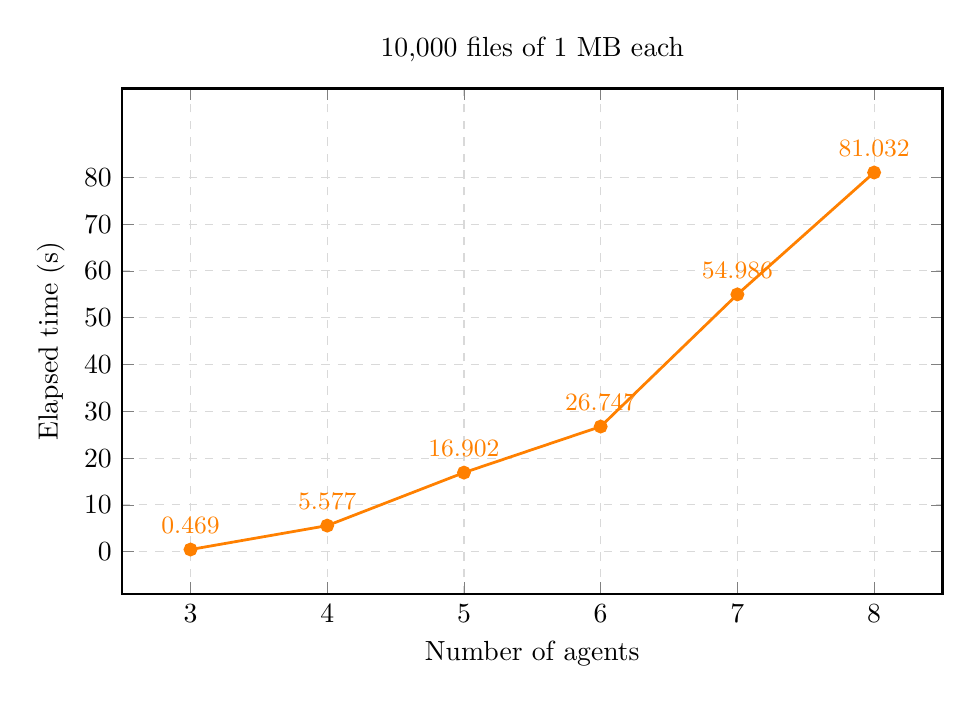
\begin{tikzpicture}
\begin{axis}[
    width=12cm, height=8cm,
    xlabel={Number of agents},
    ylabel={Elapsed time (s)},
    xmin=3, xmax=8,
    ymin=0, ymax=90,
    xtick={3,4,5,6,7,8},
    ytick={0,10,20,30,40,50,60,70,80},
    grid=major,
    grid style={dashed,gray!30},
    thick,
    title={10,000 files of 1 MB each},
    enlargelimits=0.1,
    clip=false,
    nodes near coords,
    every node near coord/.append style={font=\small, anchor=south, yshift=2pt},
    point meta=explicit symbolic
]

\addplot[color=orange, mark=*, line width=1pt] coordinates {
    (3,0.4685) [0.469]
    (4,5.577) [5.577]
    (5,16.902) [16.902]
    (6,26.747) [26.747]
    (7,54.986) [54.986]
    (8,81.032) [81.032]
};
\end{axis}
\end{tikzpicture}
\caption{Elapsed time for the corruption check with 10,000 files of 1 MB each,
    with all agents online. Each agent stores 10,000 $\times$ (1 MB / number of agents) of data.}
\label{fig:test-2}
\end{figure}

\newpage
\paragraph{Test 3: Large files, but small dataset}

This test evaluates system performance on a small dataset consisting of 10 files, each 1 GB in size, under different cluster sizes. All agents remained online during the corruption check. Figure \ref{fig:test-5} shows the elapsed time as the number of agents increases from 3 to 8. As expected, elapsed time grows with the number of agents, mainly due to shard verification and network communication overhead. The results indicate that even for small datasets, increasing cluster size introduces a modest computational cost, which remains manageable.

\begin{figure}[!ht]
\centering
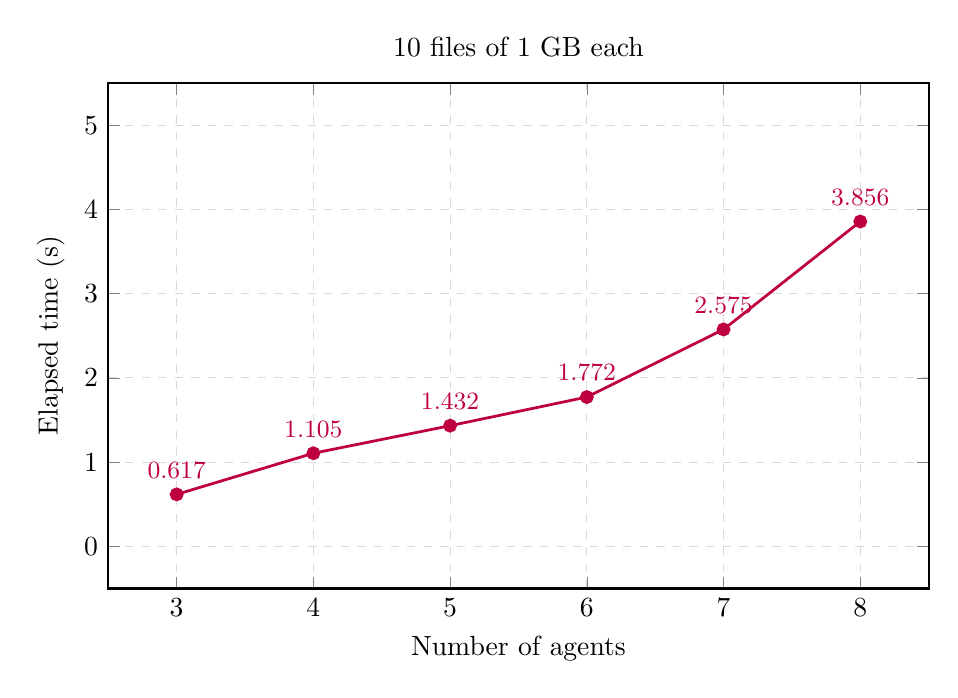
\begin{tikzpicture}
\begin{axis}[
    width=12cm, height=8cm,
    xlabel={Number of agents},
    ylabel={Elapsed time (s)},
    xmin=3, xmax=8,
    ymin=0, ymax=5,
    xtick={3,4,5,6,7,8},
    ytick={0,1,2,3,4,5},
    grid=major,
    grid style={dashed,gray!30},
    thick,
    title={10 files of 1 GB each},
    enlargelimits=0.1,
    clip=false,
    nodes near coords,
    every node near coord/.append style={font=\small, anchor=south, yshift=2pt},
    point meta=explicit symbolic
]

\addplot[color=purple, mark=*, line width=1pt] coordinates {
    (3,0.6166) [0.617]
    (4,1.105) [1.105]
    (5,1.432) [1.432]
    (6,1.772) [1.772]
    (7,2.575) [2.575]
    (8,3.856) [3.856]
};
\end{axis}
\end{tikzpicture}
\caption{Elapsed time for the corruption check with 10 files of 1 GB each, with all agents online. Each agent stores $10 \times (1 \text{ GB} / \text{number of agents})$ of data.}
\label{fig:test-5}
\end{figure}
\newpage
\paragraph{Test 4: Small files, partially offline agents}

The third scenario evaluates the effect of offline agents. 1,000 files of 150 KB
each were uploaded, and elapsed time was measured both with all agents online
and with a subset of agents offline during the corruption check.
Figure \ref{fig:test-3} compares the two configurations. Offline agents
introduce additional latency due to the timeout before retrieving the previous
saved hash, with elapsed times ranging from 28.2 to 91.338 seconds, compared to 3.1 to 69.221 seconds when all agents are online.

\begin{figure}[!ht]
\centering
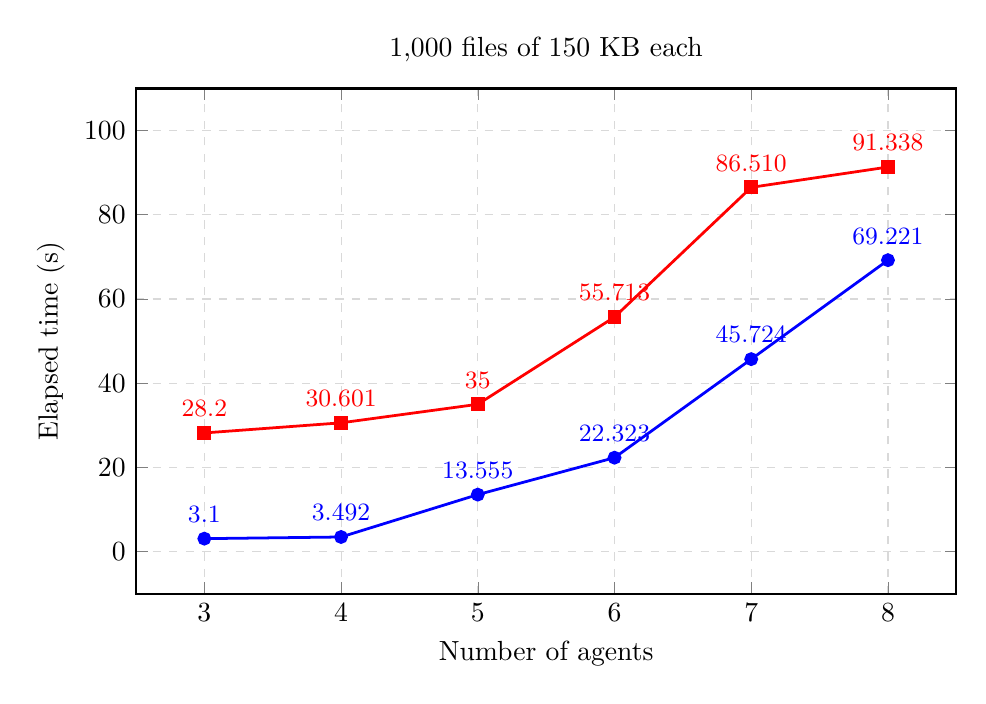
\begin{tikzpicture}
\begin{axis}[
    width=12cm, height=8cm,
    xlabel={Number of agents},
    ylabel={Elapsed time (s)},
    xmin=3, xmax=8,
    ymin=0, ymax=100,
    xtick={3,4,5,6,7,8},
    ytick={0,20,40,60,80,100},
    grid=major,
    grid style={dashed,gray!30},
    thick,
    title={1,000 files of 150 KB each},
    enlargelimits=0.1,
    clip=false,
    nodes near coords,
    every node near coord/.append style={font=\small, anchor=south, yshift=2pt},
    point meta=explicit symbolic
]

% Online agents
\addplot[color=blue, mark=*, line width=1pt] coordinates {
    (3,3.1) [3.1]
    (4,3.492) [3.492]
    (5,13.555) [13.555]
    (6,22.323) [22.323]
    (7,45.724) [45.724]
    (8,69.221) [69.221]
};

% Offline agents
\addplot[color=red, mark=square*, line width=1pt] coordinates {
    (3,28.2) [28.2]
    (4,30.601) [30.601]
    (5,35) [35]
    (6,55.713) [55.713]
    (7,86.510) [86.510]
    (8,91.338) [91.338]
};

\end{axis}
\end{tikzpicture}
\caption{Elapsed time of the corruption check with 1,000 files, each 150 KB in
    size. Each agent stores 1,000 $\times$ (150 KB / number of agents) of data. In blue with none offline agents; in red with offline
    agents.}
\label{fig:test-3}
\end{figure}

\newpage
\paragraph{Test 5: Very large number of tiny files}

The fourth test evaluates system performance with an extremely large number of very small files. The dataset consisted of one million files, distributed across different cluster configurations. Unlike the previous tests, where file sizes varied with the number of agents, in this case each file had a fixed size of 4 KB. Consequently, increasing the number of agents also increases the total global dataset size, allowing an assessment of how the system handles both a high file count and a growing overall workload.


\begin{figure}[!ht]
\centering
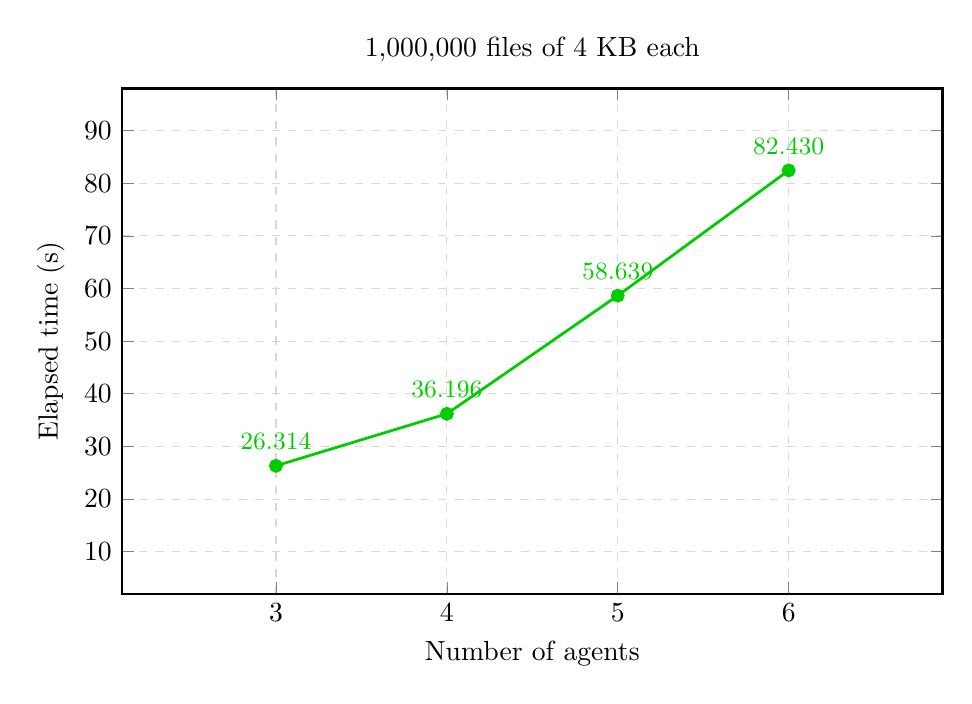
\begin{tikzpicture}
\begin{axis}[
    width=12cm, height=8cm,
    xlabel={Number of agents},
    ylabel={Elapsed time (s)},
    xmin=2.5, xmax=6.5,
    ymin=10, ymax=90,
    xtick={3,4,5,6},
    ytick={0,10,20,30,40,50,60,70,80,90,100},
    grid=major,
    grid style={dashed,gray!30},
    thick,
    title={1,000,000 files of 4 KB each},
    enlargelimits=0.1,
    clip=false,
    nodes near coords,
    every node near coord/.append style={font=\small, anchor=south, yshift=2pt},
    point meta=explicit symbolic
]

\addplot[color=green!80!black, mark=*, line width=1pt] coordinates {
    (3,26.314) [26.314]
    (4,36.196) [36.196]
    (5,58.639) [58.639]
    (6,82.430) [82.430]
};
\end{axis}
\end{tikzpicture}
\caption{Elapsed time for corruption check on very large datasets. The total dataset size increases
    with the number of agents: 12 GB for 3 agents, 16 GB for 4 agents, 20 GB
    for 5 agents, and 24 GB for 6 agents. Each agent stores 4 GB of data.}
\label{fig:test-4}
\end{figure}

\newpage

\paragraph{Results}

The experimental evaluation demonstrates that the system maintains correctness and functional reliability across a wide variety of scenarios. However, performance degrades as the cluster size increases, primarily due to the coordination and communication overhead introduced by the Raft consensus, as well as the computational cost of Merkle tree operations and network latency when retrieving root hashes from agents.

In Test 1, with 100 files of 100 MB each (10 GB total), the elapsed time increased from 1.37 s with 3 agents to 23.89 s with 8 agents. This trend shows that the system remains functional but becomes progressively slower as coordination overhead grows.

In Test 2, using 10,000 files of 1 MB each (10 GB total), elapsed time increased
from 0.47 s with 3 agents to to 81.03 s with 8 agents. This represents about
170x increase, clearly showing that scenarios with many small files amplify the cost of synchronization and consensus, leading to diminishing performance returns as the cluster expands.

Test 3, with 10 files of 1 GB each (10 GB total), exhibited a milder increase (from 0.62 s to 3.86 s) indicating that the system handles large files more efficiently. Compared to Tests 1 and 2, this suggests that performance loss is primarily driven by the number of files (and resulting coordination steps), not by total data size.

In Test 4, with 1,000 files of 150 KB each (150 MB total), the system was evaluated under partial node unavailability. When some agents were offline, execution time increased by roughly 9x (for example, from 3.1 s to 28.2 s with 3 agents). However, the relative slowdown diminished with larger clusters, confirming that Raft's fault-tolerant synchronization mitigates the effects of offline nodes, albeit at a cost in latency.

Finally, Test 5, involving one million files of 4 KB each, measured total
processing time from 26.31 s to 82.43 s as dataset size grew from 12 GB to 24
GB. Despite the large number of files, absolute latency grows and the system continues to process data at a predictable rate.

Overall, the results show that the system is robust but not performance-scalable. It preserves data integrity and correctness under varying workloads and node conditions, but verification time increases disproportionately with the number of agents and files. These findings highlight the trade-off between distributed consistency and performance in consensus-based corruption detection systems.
